\documentclass{article}
\usepackage[utf8]{inputenc}
\usepackage{amsmath,amssymb,amsthm,mathrsfs,graphicx}

\title{HW9}
\author{Ry Wiese\\wiese176@umn.edu}
\date{December 16, 2019}

\begin{document}

\maketitle

\section{Problem 1}

\subsection{Part i}

\[
\begin{array}{rrrcl}
 \min & \sum_j y_j  &      &   \\
 \mbox{s.t.}  &  \forall i,  & \sum_j x_{ij}  & = & 1~; \\
              &  \forall j  & \sum_i x_{ij}\cdot a_i & \le & V~; \\
     & \forall j, \forall i, & y_j & \ge & x_{ij}~;\\
     & \forall i, \forall j, & x_{ij}, y_j & \in & \{0,1\}.
\end{array}
\]

\subsection{Part ii}

For the IP problem, I had an optimal value of 3 bins where items 1 and 2 are in bin 1, item 3 is in bin 2, and item 4 is in bin 4. For the LP relaxation, I got an optimal value of 1 with
$\mathbf{x} = 
\left(
\begin{array}{cccc}
.25 & .25 & .25 & .25\\
.25 & .25 & .25 & .25\\
.25 & .25 & .25 & .25\\
.25 & .25 & .25 & .25\\
\end{array}
\right)
$
and
$\mathbf{y} = 
\left(
\begin{array}{c}
.25\\
.25\\
.25\\
.25\\
\end{array}
\right)
$.
This is an integrality gap of 2.

\section{Problem 2}

\subsection{Part i}

Let $S_{ij} = 1$ if customer $i$ has product $j$ in his bundle and 0 otherwise.

\[
\begin{array}{rrrcl}
 \min & & \sum_i x_i \cdot v_i\\
 \mbox{s.t.}  &  \forall j,  & \sum_i x_i \cdot S_{ij}  & \le & B_j~;\\
 & \forall i, & x_i & \in & \{0,1\}~.
\end{array}
\]

\subsection{Part ii}

For the LP relaxation and for the IP, I got an optimal solution of 8 where the seller rejects customer 1's request but accepts the other 4. The integrality gap in this case is 0.

\section{Problem 3}

I got an optimal value of 1000 with $\mathbf{x} = (1,6))$.

\begin{figure} % "h" is where to place, h=here, t=top, b=bottom
  \centering
  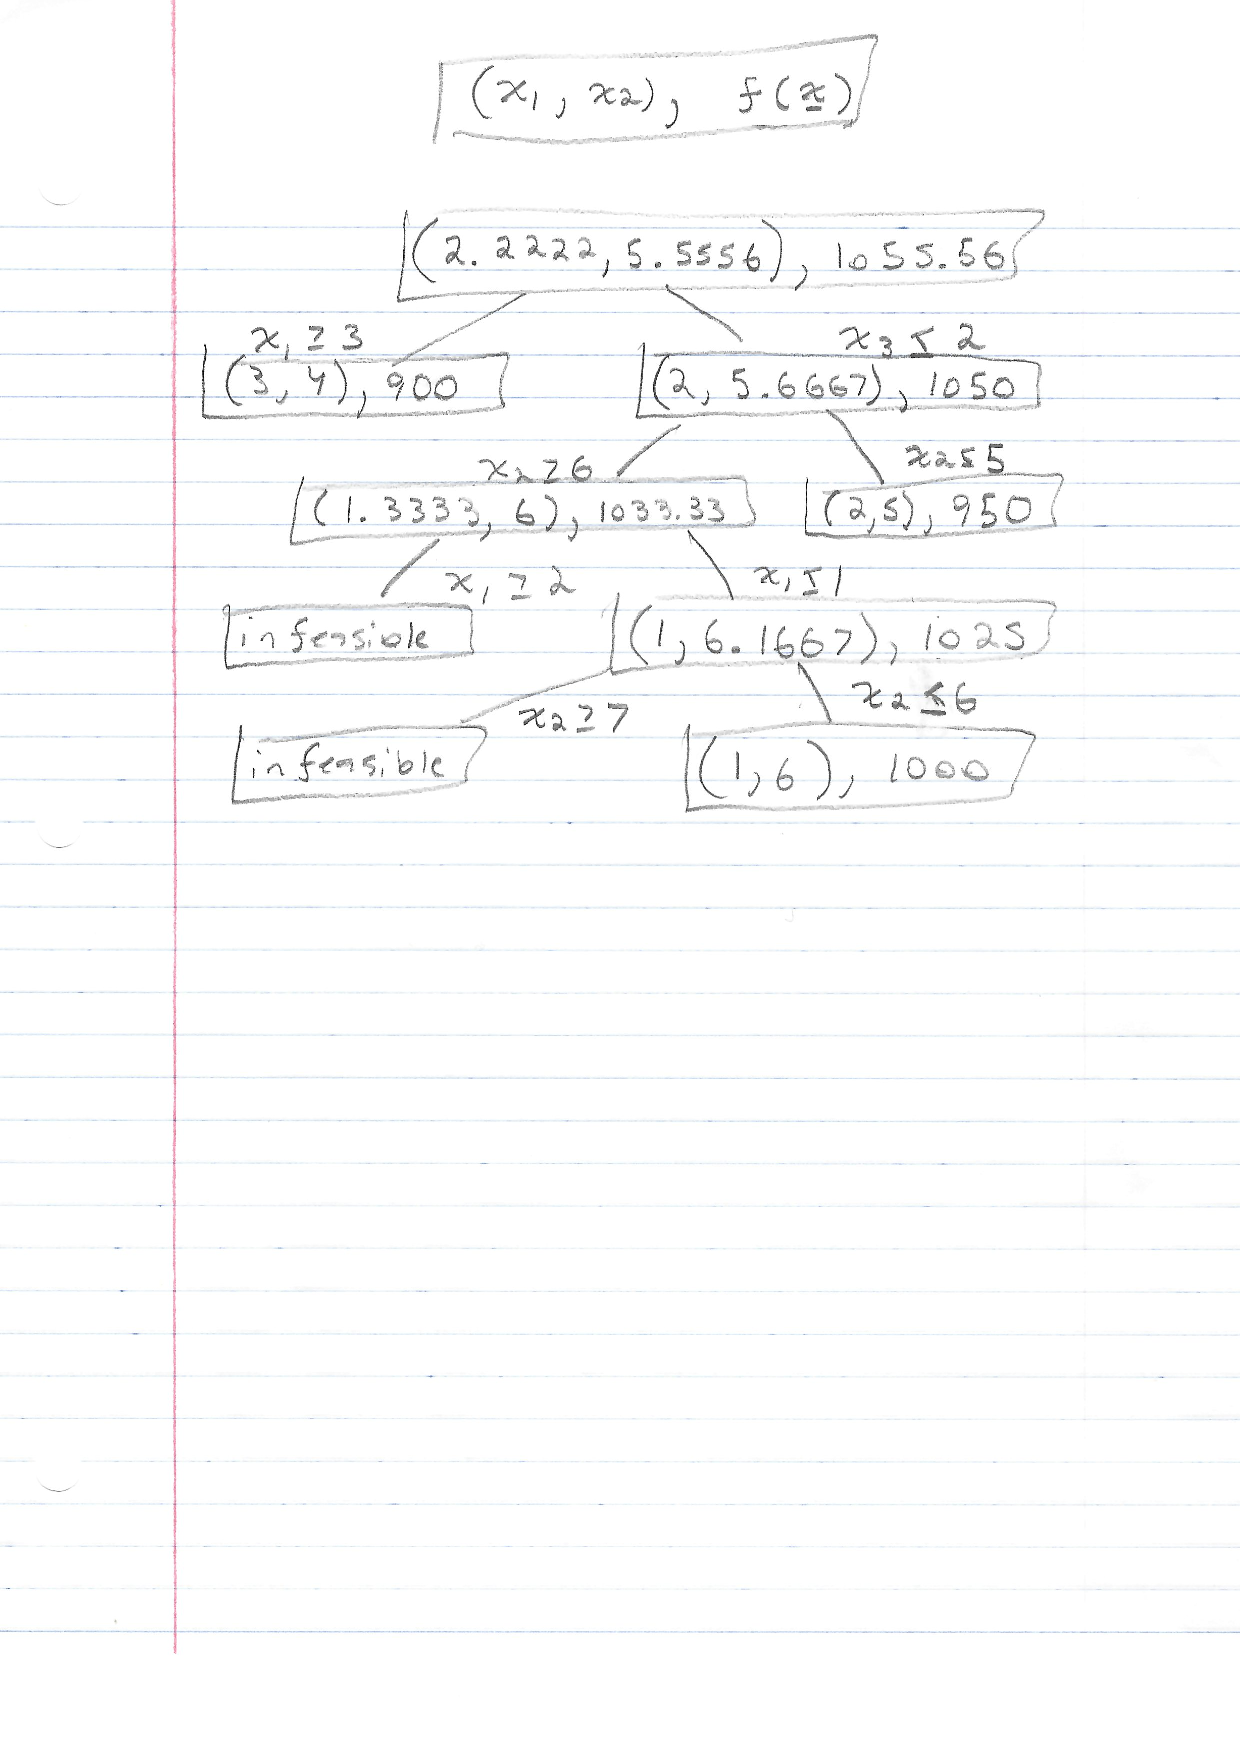
\includegraphics[angle=0,totalheight=125mm]{P3.pdf}
  \caption{Branch and Bound Tree}
  \label{fig:tabl}
\end{figure}

\end{document}
